\chapter{Another Chapter}
\lettrine[lines=1]{A}{dd} new chapters to either continue your literature review or show your solution to the problem chosen. \cite{article1}

\section{Just a section}
Keep citing the relevant papers and books and adding the BibTex format to the Content/citations.bib file. \\[4pt]
To add an image simply un-comment this thing. The width parameter specifies how wide should the picture appear on the page. You might need to adjust it to get it in the right format as you want. Don't go too small though. Try to stay between 0.6 and 1.
\begin{figure}[ht!]
    \centering
    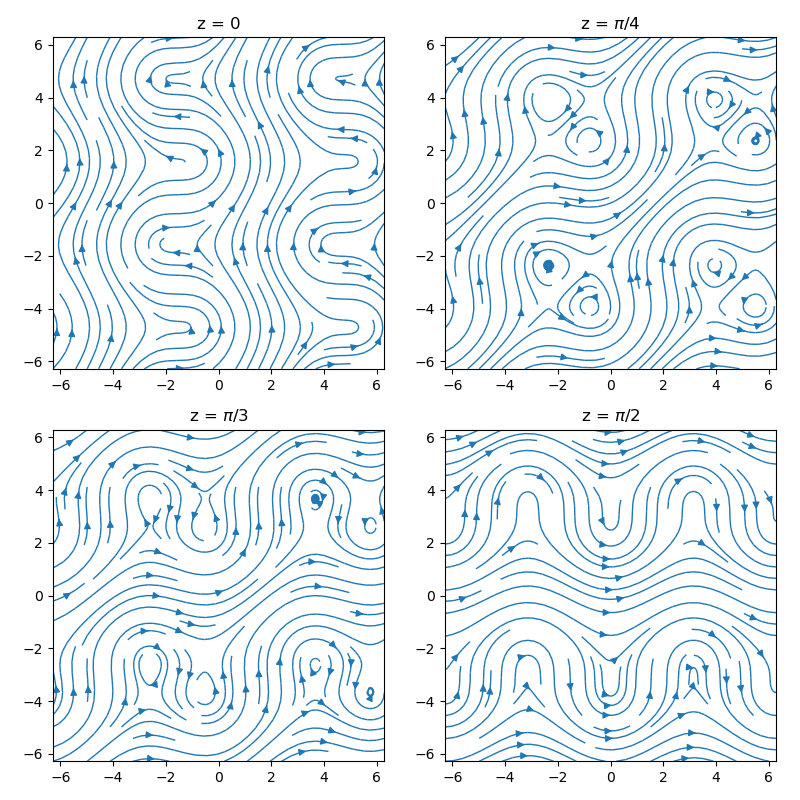
\includegraphics[width=0.7\textwidth]{Figures/ABC.png}
    \caption{Something something with $A = B = C = 0.1$ for $x, y \in [-2\pi, 2\pi]$}
    \label{ABC}
\end{figure}